\documentclass[a4paper,12pt]{article}
\usepackage[utf8]{inputenc}
\usepackage{graphicx}
\usepackage{fancyhdr}
\usepackage{amsmath}
\usepackage{adjustbox}
\usepackage{mathtools}
\usepackage{float}
\usepackage[spanish, es-nodecimaldot]{babel} 
\usepackage{lastpage}
\usepackage{amssymb} % Para símbolos matemáticos adicionales
\usepackage{hyperref}
\usepackage{cleveref}
%\usepackage[none]{hyphenat}
\usepackage{array}

\usepackage{multirow}
\usepackage{textcomp}
\usepackage[left=2.5cm, right=2.5cm, top=3cm, bottom=3cm]{geometry}

\graphicspath{{Imagenes/}}

% Encabezado y pie de página
\pagestyle{fancy}
\fancyhf{}
\setlength{\headheight}{30 pt}
\renewcommand{\headrulewidth}{0.2pt}
\fancyhead[R]{\begin{tabular}{@{}l@{}}
\includegraphics[scale=0.4]{escudo.PNG}\end{tabular}}
\fancyhead[L]{\begin{tabular}{@{}c@{}} \textbf{Robótica I - Año: 2024} \\ Trabajo Práctico 5: Cinemática Inversa \end{tabular}}


\fancyfoot[R]{\thepage}
\fancyfoot[C]{\begin{tabular}{@{}c@{}}\textbf{BORQUEZ PEREZ Juan Manuel}\\ \textbf{Legajo 13567}\end{tabular}}
\renewcommand{\footrulewidth}{0.2pt}

\begin{document}

\begin{titlepage}
    \centering
    \vspace*{5cm}
    {\Huge\bfseries Informe de Trabajo Práctico N°5}\\
    \vspace{0.2cm}
    {\Large \textbf{Cinemática Inversa}}\\
    \vspace{0.5cm}
    {\Large Robótica I}\\
    \vspace{0.5 cm}
    {\Large Ingeniería en Mecatrónica}\\
    \vspace{0.2 cm}
    {\Large Facultad de Ingeniería - UNCUYO}\\
    \vspace{1.5cm}
    Alumno: Juan Manuel BORQUEZ PEREZ\\
    Legajo: 13567\\
    \vfill
    {\begin{tabular}{@{}c@{}}
\includegraphics[scale=0.4]{escudo.PNG}\end{tabular}}\hspace{10pt}
    %Año 2023
\end{titlepage}

\section{Ejercicio 1}
\begin{figure}[H]
    \centering
    \begin{adjustbox}{scale = 0.55, max width=\columnwidth}
        \framebox{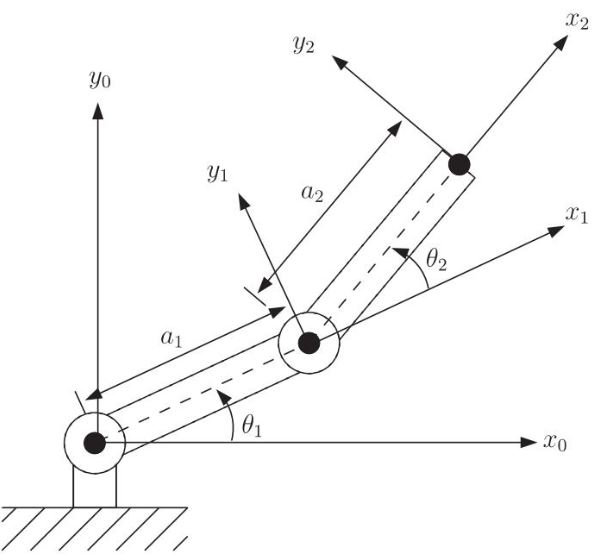
\includegraphics{1-Ejercicio_1.JPG}}
    \end{adjustbox}
    \caption{Robot Ejercicio 1}
\end{figure}

\subsection{}
\textbf{Utilice el método geométrico para hallar un conjunto de ecuaciones cerradas que resuelvan el siguiente problema}

\begin{equation*}
    \overline{q} = f\left(x,y,\gamma\right)
\end{equation*}

Al tratarse de un robot con solo dos grados de libertad, una \textbf{postura alcanzable está suficientemente definida al especificar
a lo sumo dos variables en el plano}, esto es, $\left(x,y\right)$, $\left(x,\gamma\right)$ o $\left(y, \gamma\right)$; mientras que
la tercera variable queda determinada. Luego, como el problema se formula en término de las tres variables, las mismas deben ser congruentes para
que exista solución.

Las posiciones alcanzables por el extremo del robot quedan definidas por las siguientes condiciones:
\begin{equation}
    \begin{aligned}
        \sqrt[]{x^2 + y^2 }&\leq  a_1 + a_2\,\,\, \text(extension\,maxima)\\
        \left(a_1 > a_2 \right)\rightarrow \sqrt[]{x^2 + y^2} & \geq  a_1 - a_2\,\,\, \text(extesion\,minima)
    \end{aligned}
    \label{rango}
\end{equation}

Cuando la posición es alcanzable, $\theta_2$ se puede determinar por análisis de la suma de los vectores indicados en la \cref{geometria 1}, como se indica a continuación:
\begin{align*}
    \mathbf{w} &= \mathbf{u} + \mathbf{v}\\
    \mathbf{w}^2 &= \mathbf{u}^2 + \mathbf{v}^2 + 2\mathbf{u}\cdot\mathbf{v}\\
    x^2 + y^2 &= a_{1}^2 + a_{2}^2 + 2a_{1}a_{2}\cos(\theta_2)\\
\end{align*}
Luego:
\begin{equation}
    \theta_2 = arccos\left(\frac{x^2 + y^2 - a_{1}^2 - a_{2}^2}{2a_{1}a_{2}}\right)
    \label{teta2}
\end{equation}
Esto da lugar a \textbf{dos posibles valores}, uno positivo (codo abajo) y otro negativo (codo arriba).

\begin{figure}[htbp]
    \centering
    \begin{adjustbox}{scale = 0.55, max width=\columnwidth}
        \framebox{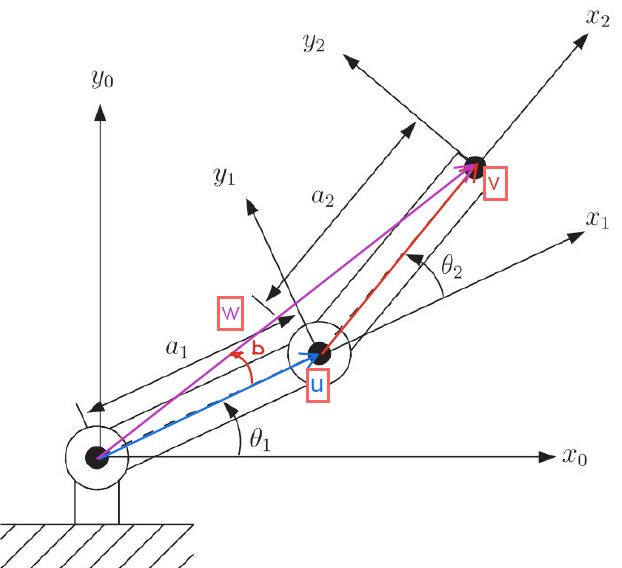
\includegraphics{2-Ejercicio_1_vectores.JPG}}
    \end{adjustbox}
    \caption{Análisis geométrico}
    \label{geometria 1}
\end{figure}

El ángulo $\theta_1$ se determina ahora por análisis de las proyecciones sobre los ejes

Sobre el eje X:
\begin{align*}
    x &= a_1\cos(\theta_1) + a_2\cos(\theta_1 + \theta_2)\\
    x &= a_1\cos(\theta_1) + a_2\left[\cos(\theta_1)\cos(\theta_2) - \sin(\theta_1)\sin(\theta_2)\right]\\
    x &= \underline{\left[a_1 + a_2\cos(\theta_2)\right]}\cos(\theta_1) - \underline{a_2\sin(\theta_2)}\sin(\theta_1)\\
    x &= \underline{A}\cos(\theta_1) - \underline{B}\sin(\theta_1)
\end{align*}
Sobre el eje Y:
\begin{align*}
    y &= a_1\sin(\theta_1) + a_2\sin(\theta_1 + \theta_2)\\
    y &= a_1\sin(\theta_1) + a_2\left[\sin(\theta_1)\cos(\theta_2) + \cos(\theta_1)\sin(\theta_2)\right]\\
    y &= \underline{\left[a_1 + a_2\cos(\theta_2)\right]}\sin(\theta_1) + \underline{a_2\sin(\theta_2)}\cos(\theta_1)\\
    y &= \underline{A}\sin(\theta_1) + \underline{B}\cos(\theta_1)
\end{align*}
Se obtiene el siguiente sistema de ecuaciones lineales:
\begin{align*}
    \begin{cases}
        x &= A\cos(\theta_1) - B\sin(\theta_1)\\
        y &= B\cos(\theta_1) + A\sin(\theta_1)
    \end{cases}
\end{align*}
Entonces se puede obtener $\theta_1$ a partir de las siguientes:
\begin{align}
    \begin{cases}
        \cos(\theta_1) &= \frac{Ax + By}{A^2 + B^2}\\
        \sin(\theta_1) &= \frac{Ay - Bx}{A^2 + B^2}\\
        \theta_1 &= \arctan{\left(\frac{Ay - Bx}{Ax + By}\right) = atan2(Ay-Bx, Ax + By)}
    \end{cases}
    \label{teta1}
\end{align}
La última se utiliza para determinar dos posibles soluciones para $\theta_1$ mientras que el signo de las primeras dos determinan el valor correcto (el cuadrante).
La \cref{teta1} se resuleve para cada valor de B (uno por cada valor de $\theta_2$ dados en la \cref{teta2}).

Finalmente, la orientación dada para la postura en la formulación del problema debe ser congruente, y esta dada por:
\[\gamma = \theta_1 + \theta_2\]

En resumen, para $\overline{q} = (x, y, \gamma)$ en el rango del robot según \cref{rango} se obtiene un par de posibles soluciones (codo arriba y codo abajo) dadas por:
\begin{align}
    \begin{cases}
        \theta_2 &= arccos\left(\frac{x^2 + y^2 - a_{1}^2 - a_{2}^2}{2a_{1}a_{2}}\right) \rightarrow A = a_1 + a_2\cos(\theta_2); B = a_2\sin(\theta_2)\\
        \theta_1 &=  atan2(Ay-Bx, Ax + By)\\
        \overline{q} &= (\theta_1, \theta_2)\\
        \text{solo\,si}\,\,\gamma &= \theta_1 + \theta_2
    \end{cases}
\end{align}
En los extremos del movimiento del robot se puede obtener a lo sumo una solución (no un par).



\subsection{}
\textbf{Utilice el método geométrico para hallar un conjunto de ecuaciones cerradas que resuelvan el siguiente problema}

\begin{equation*}
    \overline{q} = f\left(x,y\right)
\end{equation*}
La solución es la misma que en el caso anterior solamente que en este caso la orientación queda determinada por los desplazamientos angulares obtenidos:
\begin{align}
    \begin{cases}
        \theta_2 &= arccos\left(\frac{x^2 + y^2 - a_{1}^2 - a_{2}^2}{2a_{1}a_{2}}\right) \rightarrow A = a_1 + a_2\cos(\theta_2); B = a_2\sin(\theta_2)\\
        \theta_1 &=  atan2(Ay-Bx, Ax + By)\\
        \overline{q} &= (\theta_1, \theta_2)
    \end{cases}
\end{align}

\subsection{}
\textbf{Indique la cantidad de soluciones posibles que tendría cada conjunto de ecuaciones anterior, si los límites articulares fueran los siguientes}
\subsubsection{$\pm 90^\circ$}
La mínima extensión alcanzable por el robot se consigue cuando los eslabones forman un ángulo recto. Luego la condición de rango señalada en \cref{rango} es ahora:
\begin{equation}
    \begin{aligned}
        \sqrt{x^2 + y^2}&\leq  a_1 + a_2\,\,\, \text(extension\,maxima)\\
        x^2 + y^2& \geq a_1^2 + a_2^2\,\,\, \text(extension\,minima)
    \end{aligned}
    \label{rango 90}
\end{equation}

Para los puntos dentro del rango del robot, definido en \cref{rango 90}, y analizando \cref{teta1} vemos que tendremos dos posibles soluciones (codo arriba y codo abajo)
siempre que para ambos valores de $\theta_2$ en el rango articular sea $Ay-Bx \geq 0$, habrá una única solución cuando solo para uno de los valores de $\theta_2$ la desigualdad de un valor positivo
y no habrá soluciones cuando para ambos valores de $\theta_2$ la desigualdad de valores negativos.

\subsubsection{$\pm 180^\circ$}
\subsubsection{$\pm 225^\circ$}
\subsubsection{$\pm \infty$}

%\begin{equation*}
%    \prescript{O}{}{Rot_M} = 
%    \begin{bmatrix}
%        0.500 & -0.866\\
%        0.866 & 0.500
%    \end{bmatrix}
%\end{equation*}

%\begin{figure}[H]
%    \centering
%    \begin{adjustbox}{scale = 0.85, max width=\columnwidth}
%        \framebox{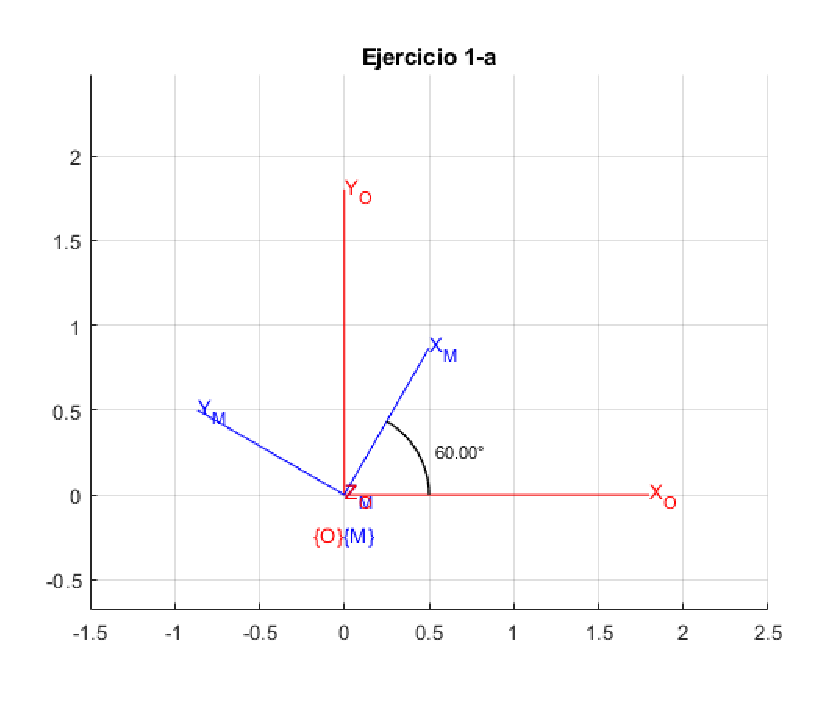
\includegraphics{1-Ejercicio_1_a.pdf}}
%    \end{adjustbox}
%    \caption{Sistema O y Sistema M superpuestos con indicación de ángulo de rotación.}
%\end{figure}


%\begin{table}[H]
%    \centering
%    \begin{tabular}{|c|c|c|c|c|c|}
%    \hline
%    Sistema & $\theta$  & $d$           & $a$    & $\alpha$ & $\sigma$ \\ \hline
%    1       & $q_1$     & $199.2$       & $200$  & 0        & 0        \\ \hline
%    2       & $q_2$     & $59.5$        & $250$  & 0        & 0        \\ \hline
%    3       & $0$       & $q_3$         & $0$    & 180°     & 1        \\ \hline
%    4       & $q_4$     & $37.5$        & $0$    & 0        & 0        \\ \hline
%    \end{tabular}
%    \caption{Parámetros DH alternativos.}
%    \label{parametros DH2}
%\end{table}

\end{document}